% ============================================
% SECTION: SINGLE RESPONSIBILITY PRINCIPLE
% ============================================

\section{Single Responsibility Principle (SRP)}

\subsection{Definition of SRP}

The Single Responsibility Principle (SRP) is one of the five SOLID principles of object-oriented design, introduced by Robert C. Martin. It states that \textit{``a class should have one, and only one, reason to change.''} In other words, each class should have a single responsibility or purpose, focusing on one specific aspect of the software's functionality. This principle ensures that a class is cohesive and that changes to one part of the system do not inadvertently affect unrelated functionality.

\subsection{Importance of SRP in Object-Oriented Design}

SRP is fundamental to creating maintainable, scalable, and robust software systems. Its importance can be understood through several key benefits:

\begin{itemize}
    \item \textbf{Improved Maintainability:} When each class has a single responsibility, changes to one aspect of the system are isolated to specific classes, making the codebase easier to understand and modify.
    
    \item \textbf{Enhanced Testability:} Classes with a single responsibility are simpler to test, as they have fewer dependencies and a more focused scope. Unit tests become more straightforward and reliable.
    
    \item \textbf{Reduced Coupling:} By separating concerns, SRP reduces the dependencies between different parts of the system, making the code more modular and flexible.
    
    \item \textbf{Better Reusability:} Classes designed with a single purpose can be more easily reused in different contexts without bringing along unnecessary functionality.
    
    \item \textbf{Easier Collaboration:} When responsibilities are clearly separated, different team members can work on different parts of the system without interfering with each other's work.
\end{itemize}

\subsection{Exercise Analysis: Car Management System}

\subsubsection{Description of the Original Design (Before Refactoring)}

The original exercise presents a \texttt{CarManager} class responsible for managing car-related operations. This class handles three distinct responsibilities:

\begin{enumerate}
    \item \textbf{Data Access:} Managing the car database (a hardcoded list) and retrieving cars by ID through the \texttt{getFromDb(String carId)} method.
    
    \item \textbf{Presentation Logic:} Formatting car information for display through the \texttt{getCarsNames()} method, which concatenates car brands and models into a comma-separated string.
    
    \item \textbf{Business Logic:} Determining the ``best'' car based on lexicographical comparison of model names through the \texttt{getBestCar()} method.
\end{enumerate}

The \texttt{Car} class serves as a simple data model with three attributes: \texttt{\_id}, \texttt{\_model}, and \texttt{\_brand}, along with their corresponding getter methods.

\subsubsection{Identified SRP Violations}

The original design violates the Single Responsibility Principle in several ways:

\begin{itemize}
    \item \textbf{Multiple Reasons to Change:} The \texttt{CarManager} class would need to be modified if:
    \begin{itemize}
        \item The data source changes (e.g., from in-memory list to database)
        \item The formatting requirements change (e.g., different output format)
        \item The selection criteria for ``best car'' changes (e.g., based on price instead of model name)
    \end{itemize}
    
    \item \textbf{High Coupling:} The class is tightly coupled to both the data structure and the presentation format, making it difficult to modify one aspect without affecting others.
    
    \item \textbf{Poor Testability:} Testing individual responsibilities (data access, formatting, or selection logic) requires testing the entire class, making unit tests more complex and fragile.
    
    \item \textbf{Code Duplication Risk:} If similar formatting or data access is needed elsewhere in the application, the logic would likely be duplicated rather than reused.
\end{itemize}

\subsubsection{UML Diagram of the Original Design}

\begin{figure}[H]
    \centering
    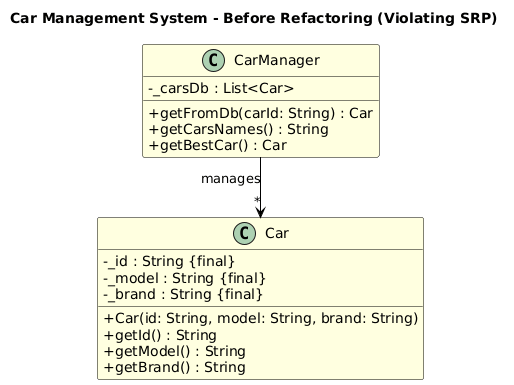
\includegraphics[width=0.6\textwidth]{SRP/plantUML/before.png}
    \caption{UML Diagram - Car Management System Before Refactoring}
    \label{fig:srp_before}
\end{figure}

Figure~\ref{fig:srp_before} illustrates the original design where \texttt{CarManager} contains multiple responsibilities within a single class, violating the Single Responsibility Principle.

\subsection{Refactored Solution}

\subsubsection{Overview of the Refactoring Approach}

To align with the Single Responsibility Principle, the design was refactored to separate the distinct responsibilities into dedicated classes. The refactoring introduces the following components:

\begin{enumerate}
    \item \textbf{Car:} Remains as a pure data model with no additional responsibilities.
    
    \item \textbf{CarRepository (Interface):} Defines the contract for data access operations, promoting loose coupling and testability.
    
    \item \textbf{InMemoryCarRepository:} Implements the \texttt{CarRepository} interface, encapsulating all data access logic and storage management.
    
    \item \textbf{CarFormatter:} Handles all presentation and formatting logic for car information.
    
    \item \textbf{CarService:} Contains the business logic for determining the best car based on specific criteria.
    
    \item \textbf{Client:} Serves as the application entry point, orchestrating the interaction between different components without containing business logic.
\end{enumerate}

\subsubsection{Detailed Explanation of Each Component}

\paragraph{Car - The Model}

The \texttt{Car} class remains unchanged as it already adheres to SRP. It serves solely as a data container with three immutable fields (\texttt{\_id}, \texttt{\_model}, \texttt{\_brand}) and their corresponding getter methods.

\textbf{Responsibility:} Representing car data.

\textbf{Reason to change:} Only if the car data structure itself needs to be modified (e.g., adding new attributes like year or price).

\paragraph{CarRepository - The Data Access Interface}

\begin{verbatim}
public interface CarRepository {
    Car findById(String id);
    List<Car> findAll();
}
\end{verbatim}

\textbf{Design Decision:} Using an interface rather than a concrete class provides several advantages:
\begin{itemize}
    \item \textbf{Dependency Inversion:} Higher-level modules depend on abstractions rather than concrete implementations.
    \item \textbf{Flexibility:} Easy to swap implementations (e.g., from in-memory to database) without affecting dependent classes.
    \item \textbf{Testability:} Allows for easy mocking in unit tests.
\end{itemize}

\textbf{Responsibility:} Defining the contract for car data access.

\textbf{Reason to change:} Only if the data access contract needs to be modified (e.g., adding new query methods).

\paragraph{InMemoryCarRepository - The Data Access Implementation}

\begin{verbatim}
public class InMemoryCarRepository implements CarRepository {
    private final List<Car> _cars = Arrays.asList(
        new Car("1", "Golf III", "Volkswagen"),
        new Car("2", "Multipla", "Fiat"),
        new Car("3", "Megane", "Renault")
    );
    
    @Override
    public Car findById(String id) {
        for (Car car : _cars) {
            if (car.getId().equals(id)) {
                return car;
            }
        }
        return null;
    }
    
    @Override
    public List<Car> findAll() {
        return _cars;
    }
}
\end{verbatim}

\textbf{Design Decision:} This class encapsulates all data storage and retrieval logic. The hardcoded list is now isolated in this single class.

\textbf{Responsibility:} Managing car data storage and retrieval in memory.

\textbf{Reason to change:} Only if the data storage mechanism changes (e.g., connecting to a database, reading from a file).

\textbf{Benefits:}
\begin{itemize}
    \item Data source changes are isolated to this class
    \item Can be easily replaced with \texttt{DatabaseCarRepository} or \texttt{FileCarRepository}
    \item Other classes remain unaffected by data access changes
\end{itemize}

\paragraph{CarFormatter - The Presentation Layer}

\begin{verbatim}
public class CarFormatter {
    public String formatCarNames(List<Car> cars) {
        StringBuilder sb = new StringBuilder();
        for (Car car : cars) {
            sb.append(formatCarName(car));
            sb.append(", ");
        }
        return sb.substring(0, sb.length() - 2);
    }
    
    public String formatCarName(Car car) {
        return car.getBrand() + " " + car.getModel();
    }
}
\end{verbatim}

\textbf{Design Decision:} All formatting and presentation logic is centralized in this class. It provides both individual car formatting and list formatting methods.

\textbf{Responsibility:} Formatting car information for display.

\textbf{Reason to change:} Only if the presentation format needs to be modified (e.g., changing from ``Brand Model'' to ``Model (Brand)'', or exporting to JSON/XML).

\textbf{Benefits:}
\begin{itemize}
    \item Formatting logic can be changed without affecting data access or business logic
    \item Easy to add new formatting methods (e.g., \texttt{toJSON()}, \texttt{toXML()})
    \item Formatting can be tested independently
    \item Can be reused across different parts of the application
\end{itemize}

\paragraph{CarService - The Business Logic Layer}

\begin{verbatim}
public class CarService {
    private final CarRepository _repository;
    
    public CarService(CarRepository repository) {
        _repository = repository;
    }
    
    public Car getBestCar() {
        List<Car> cars = _repository.findAll();
        Car bestCar = null;
        for (Car car : cars) {
            if (bestCar == null || 
                car.getModel().compareTo(bestCar.getModel()) > 0) {
                bestCar = car;
            }
        }
        return bestCar;
    }
}
\end{verbatim}

\textbf{Design Decision:} This class focuses exclusively on business logic—determining which car is ``best'' according to specific criteria.

\textbf{Responsibility:} Implementing business rules for car selection.

\textbf{Reason to change:} Only if the business logic for determining the best car changes (e.g., selecting based on brand popularity, price, or user ratings).

\textbf{Benefits:}
\begin{itemize}
    \item Business logic is isolated and easy to modify
    \item Can be tested independently with mock repositories
    \item Selection criteria changes don't affect data access or presentation
    \item Constructor injection allows for flexible repository implementations
\end{itemize}

\paragraph{Client - The Orchestrator}

\begin{verbatim}
public class Client {
    public static void main(String[] args) {
        // Initialize dependencies
        CarRepository repository = new InMemoryCarRepository();
        CarFormatter formatter = new CarFormatter();
        CarService service = new CarService(repository);
        
        // Display all car names
        List<Car> allCars = repository.findAll();
        String carsNames = formatter.formatCarNames(allCars);
        System.out.println("All Cars: " + carsNames);
        
        // Display best car
        Car bestCar = service.getBestCar();
        if (bestCar != null) {
            System.out.println("Best Car: " + 
                formatter.formatCarName(bestCar));
        }
        
        // Display car by ID
        Car carById = repository.findById("2");
        if (carById != null) {
            System.out.println("Car with ID 2: " + 
                formatter.formatCarName(carById));
        }
    }
}
\end{verbatim}

\textbf{Design Decision:} The \texttt{Client} class serves as the application entry point, coordinating the interaction between components without implementing business logic itself.

\textbf{Responsibility:} Application workflow orchestration and component wiring.

\textbf{Reason to change:} Only if the application workflow or component interaction pattern changes.

\textbf{Benefits:}
\begin{itemize}
    \item Clear separation between coordination and implementation
    \item Easy to understand the application flow
    \item Components can be tested independently of the orchestration
    \item Demonstrates dependency injection pattern
\end{itemize}

\subsubsection{UML Diagram of the Refactored Design}

\begin{figure}[H]
    \centering
    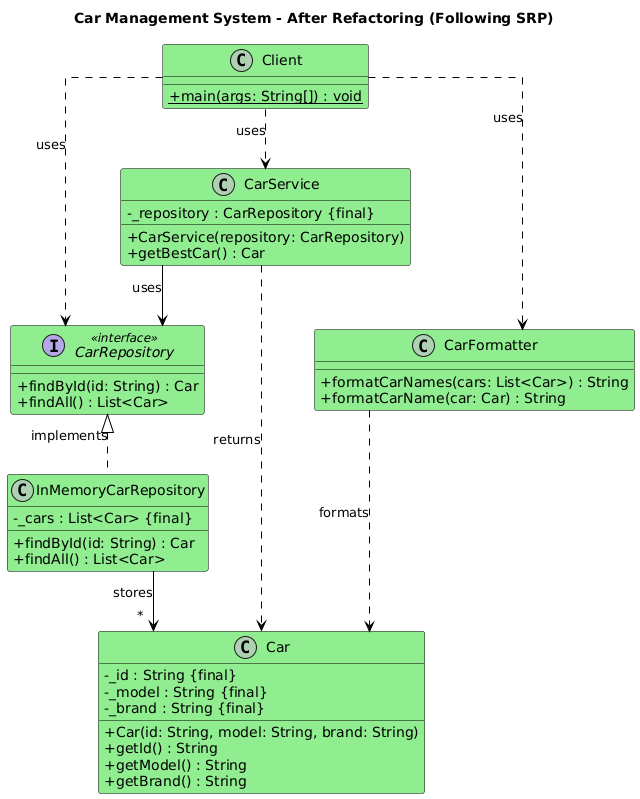
\includegraphics[width=0.9\textwidth]{SRP/plantUML/after.png}
    \caption{UML Diagram - Car Management System After Refactoring}
    \label{fig:srp_after}
\end{figure}

Figure~\ref{fig:srp_after} illustrates the refactored design where each class has a single, well-defined responsibility. The diagram shows clear separation of concerns through the use of interfaces and dedicated classes.

\subsection{How the Refactoring Aligns with SRP}

The refactored design successfully adheres to the Single Responsibility Principle through the following improvements:

\subsubsection{Single Reason to Change}

Each class now has exactly one reason to change:

\begin{table}[H]
\centering
\begin{tabular}{|l|p{8cm}|}
\hline
\textbf{Class} & \textbf{Reason to Change} \\
\hline
Car & Car data structure changes \\
\hline
CarRepository & Data access contract changes \\
\hline
InMemoryCarRepository & Data storage mechanism changes \\
\hline
CarFormatter & Presentation format changes \\
\hline
CarService & Business logic for selection changes \\
\hline
Client & Application workflow changes \\
\hline
\end{tabular}
\caption{Single Responsibility Mapping}
\label{tab:srp_responsibilities}
\end{table}

\subsubsection{Reduced Coupling}

The refactored design significantly reduces coupling:

\begin{itemize}
    \item \textbf{CarService} depends only on the \texttt{CarRepository} interface, not concrete implementations
    \item \textbf{CarFormatter} has no dependencies on other components
    \item \textbf{Client} coordinates components but doesn't implement their logic
    \item Each component can be modified independently without affecting others
\end{itemize}

\subsubsection{Improved Testability}

Each component can now be tested in isolation:

\begin{itemize}
    \item \textbf{InMemoryCarRepository:} Test data retrieval logic without business or presentation logic
    \item \textbf{CarFormatter:} Test formatting independently with sample \texttt{Car} objects
    \item \textbf{CarService:} Test business logic with a mock repository
    \item Unit tests are simpler, faster, and more focused
\end{itemize}

\subsubsection{Enhanced Maintainability}

The refactored design improves maintainability:

\begin{itemize}
    \item Changes are localized to specific classes
    \item New features can be added without modifying existing code
    \item Code is more readable with clear class names indicating purpose
    \item Dependencies are explicit and manageable
\end{itemize}

\subsubsection{Better Scalability}

The design scales well with new requirements:

\begin{itemize}
    \item \textbf{New data sources:} Add \texttt{DatabaseCarRepository} implementing \texttt{CarRepository}
    \item \textbf{New formats:} Add methods to \texttt{CarFormatter} or create specialized formatters
    \item \textbf{New selection criteria:} Modify \texttt{CarService} or create new service classes
    \item Each addition follows the same principle of single responsibility
\end{itemize}

\subsection{Conclusion}

The refactoring from a monolithic \texttt{CarManager} class to a well-structured set of classes demonstrates the power of the Single Responsibility Principle. By ensuring that each class has one reason to change, we've created a system that is:

\begin{itemize}
    \item More maintainable and easier to understand
    \item More testable with isolated unit tests
    \item More flexible and adaptable to change
    \item Better organized with clear separation of concerns
    \item More reusable with modular components
\end{itemize}

This transformation shows that SRP is not just a theoretical concept but a practical approach to building robust, professional software systems.

% ============================================
% SECTION: OPEN-CLOSED PRINCIPLE
% ============================================

\section{Open-Closed Principle (OCP)}

\subsection{Definition of OCP}

The Open-Closed Principle (OCP) is one of the five SOLID principles of object-oriented design, formulated by Bertrand Meyer. It states that \textit{``software entities (classes, modules, functions, etc.) should be open for extension but closed for modification.''} This means that the behavior of a module should be extendable to accommodate new requirements or features without altering its existing source code. In essence, you should be able to add new functionality by writing new code rather than changing existing, tested code.

\subsection{Importance of OCP in Object-Oriented Design}

The Open-Closed Principle is crucial for building maintainable and scalable software systems. Its significance can be understood through several key benefits:

\begin{itemize}
    \item \textbf{Reduced Risk of Bugs:} By avoiding modifications to existing, tested code, you minimize the risk of introducing new bugs or breaking existing functionality.
    
    \item \textbf{Enhanced Stability:} Closed modules provide a stable foundation that other parts of the system can depend on without fear of unexpected changes.
    
    \item \textbf{Improved Scalability:} Systems designed with OCP can grow by adding new components rather than continuously modifying existing ones, making long-term maintenance easier.
    
    \item \textbf{Better Code Reusability:} Well-designed abstractions can be reused across different contexts without modification.
    
    \item \textbf{Simplified Testing:} New extensions can be tested independently without retesting the entire existing codebase.
    
    \item \textbf{Easier Collaboration:} Team members can add new features by creating new classes without interfering with existing code that others might be working on.
\end{itemize}

\subsection{Exercise Analysis: Resource Allocator System}

\subsubsection{Description of the Original Design (Before Refactoring)}

The original exercise presents a \texttt{ResourceAllocator} class responsible for allocating and freeing different types of resources. The system handles two resource types defined in a \texttt{ResourceType} enum: \texttt{TIME\_SLOT} and \texttt{SPACE\_SLOT}.

The \texttt{ResourceAllocator} class contains:

\begin{itemize}
    \item \textbf{Public methods:}
    \begin{itemize}
        \item \texttt{int allocate(ResourceType resourceType)}: Allocates a resource based on its type
        \item \texttt{void free(ResourceType resourceType, int resourceId)}: Frees a previously allocated resource
    \end{itemize}
    
    \item \textbf{Private methods for time slots:}
    \begin{itemize}
        \item \texttt{int findFreeTimeSlot()}: Finds an available time slot
        \item \texttt{void markTimeSlotBusy(int resourceId)}: Marks a time slot as occupied
        \item \texttt{void markTimeSlotFree(int resourceId)}: Marks a time slot as available
    \end{itemize}
    
    \item \textbf{Private methods for space slots:}
    \begin{itemize}
        \item \texttt{int findFreeSpaceSlot()}: Finds an available space slot
        \item \texttt{void markSpaceSlotBusy(int resourceId)}: Marks a space slot as occupied
        \item \texttt{void markSpaceSlotFree(int resourceId)}: Marks a space slot as available
    \end{itemize}
\end{itemize}

Both public methods use \texttt{switch} statements to determine which resource type is being requested and call the appropriate private methods.

\subsubsection{Identified OCP Violations}

The original design violates the Open-Closed Principle in several critical ways:

\begin{itemize}
    \item \textbf{Not Open for Extension:} Adding a new resource type (e.g., \texttt{NETWORK\_SLOT}) requires:
    \begin{enumerate}
        \item Modifying the \texttt{ResourceType} enum
        \item Adding a new case to the \texttt{switch} statement in \texttt{allocate()}
        \item Adding a new case to the \texttt{switch} statement in \texttt{free()}
        \item Adding three new private methods: \texttt{findFreeNetworkSlot()}, \texttt{markNetworkSlotBusy()}, and \texttt{markNetworkSlotFree()}
    \end{enumerate}
    
    \item \textbf{Not Closed for Modification:} Every new resource type forces modification of the \texttt{ResourceAllocator} class, violating the ``closed for modification'' principle.
    
    \item \textbf{Tight Coupling:} The \texttt{ResourceAllocator} is tightly coupled to specific resource types, making it impossible to add new types without changing the class.
    
    \item \textbf{Code Duplication:} The pattern of finding free slots and marking them busy/free is repeated for each resource type, leading to code duplication.
    
    \item \textbf{Poor Scalability:} As the number of resource types grows, the \texttt{ResourceAllocator} class becomes increasingly complex and harder to maintain.
    
    \item \textbf{Violation of SRP:} The class has multiple reasons to change—once for each resource type's logic, further compounding the design issues.
    
    \item \textbf{Testing Complexity:} Every new resource type requires retesting the entire \texttt{ResourceAllocator} class, including existing functionality.
\end{itemize}

\subsubsection{UML Diagram of the Original Design}

\begin{figure}[H]
    \centering
    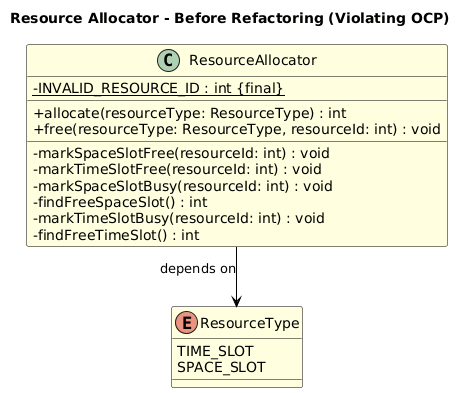
\includegraphics[width=0.7\textwidth]{OCP/plantUML/before.png}
    \caption{UML Diagram - Resource Allocator Before Refactoring}
    \label{fig:ocp_before}
\end{figure}

Figure~\ref{fig:ocp_before} illustrates the original design where \texttt{ResourceAllocator} is tightly coupled to \texttt{ResourceType} and contains all resource-specific logic within a single class, violating the Open-Closed Principle.

\subsection{Refactored Solution}

\subsubsection{Overview of the Refactoring Approach}

To align with the Open-Closed Principle, the design was refactored to introduce polymorphism and abstraction. The key insight is to encapsulate resource-specific behavior into separate classes that implement a common interface. The refactoring introduces the following components:

\begin{enumerate}
    \item \textbf{Resource (Interface):} Defines the contract that all resource types must implement.
    
    \item \textbf{TimeSlotResource:} Implements the \texttt{Resource} interface with time slot-specific logic.
    
    \item \textbf{SpaceSlotResource:} Implements the \texttt{Resource} interface with space slot-specific logic.
    
    \item \textbf{ResourceAllocator:} Simplified class that works with the \texttt{Resource} interface, delegating to specific implementations.
    
    \item \textbf{Client:} Demonstrates how to use the system and shows the extensibility benefits.
\end{enumerate}

\subsubsection{Detailed Explanation of Each Component}

\paragraph{Resource - The Abstraction}

\begin{verbatim}
public interface Resource {
    int allocate();
    void free(int resourceId);
}
\end{verbatim}

\textbf{Design Decision:} The \texttt{Resource} interface defines the contract that all concrete resource types must fulfill. By programming to an interface rather than concrete implementations, we enable polymorphism and achieve the core of OCP.

\textbf{Key Characteristics:}
\begin{itemize}
    \item \textbf{Simple Contract:} Only two methods define the essential operations any resource must support
    \item \textbf{No Implementation:} The interface contains no implementation details, leaving them to concrete classes
    \item \textbf{Stable Interface:} Once defined, this interface rarely needs to change, making it ``closed for modification''
    \item \textbf{Extensible:} New resource types can be added by implementing this interface without changing existing code
\end{itemize}

\textbf{Benefits:}
\begin{itemize}
    \item Provides a stable abstraction for the \texttt{ResourceAllocator} to depend on
    \item Enables polymorphic behavior—different resources can be treated uniformly
    \item Facilitates testing through mock implementations
    \item Documents the contract that all resources must fulfill
\end{itemize}

\paragraph{TimeSlotResource - Time Slot Implementation}

\begin{verbatim}
public class TimeSlotResource implements Resource {
    @Override
    public int allocate() {
        int resourceId = findFreeTimeSlot();
        markTimeSlotBusy(resourceId);
        return resourceId;
    }
    
    @Override
    public void free(int resourceId) {
        markTimeSlotFree(resourceId);
    }
    
    private int findFreeTimeSlot() {
        return 0;
    }
    
    private void markTimeSlotBusy(int resourceId) {
        System.out.println("Time slot " + resourceId + 
            " marked as busy");
    }
    
    private void markTimeSlotFree(int resourceId) {
        System.out.println("Time slot " + resourceId + 
            " marked as free");
    }
}
\end{verbatim}

\textbf{Design Decision:} This class encapsulates all logic specific to time slot resources. It implements the \texttt{Resource} interface and provides concrete implementations for allocation and deallocation.

\textbf{Responsibility:} Managing time slot resource lifecycle (finding, allocating, freeing).

\textbf{Key Characteristics:}
\begin{itemize}
    \item \textbf{Encapsulation:} All time slot logic is contained within this class
    \item \textbf{Self-contained:} Manages its own state and behavior
    \item \textbf{Private helpers:} Uses private methods for internal operations
    \item \textbf{No external dependencies:} Can operate independently
\end{itemize}

\textbf{Benefits:}
\begin{itemize}
    \item Time slot logic can be modified without affecting other resource types
    \item Can be tested independently
    \item Clear responsibility and purpose
    \item Easy to understand and maintain
\end{itemize}

\paragraph{SpaceSlotResource - Space Slot Implementation}

\begin{verbatim}
public class SpaceSlotResource implements Resource {
    @Override
    public int allocate() {
        int resourceId = findFreeSpaceSlot();
        markSpaceSlotBusy(resourceId);
        return resourceId;
    }
    
    @Override
    public void free(int resourceId) {
        markSpaceSlotFree(resourceId);
    }
    
    private int findFreeSpaceSlot() {
        return 0;
    }
    
    private void markSpaceSlotBusy(int resourceId) {
        System.out.println("Space slot " + resourceId + 
            " marked as busy");
    }
    
    private void markSpaceSlotFree(int resourceId) {
        System.out.println("Space slot " + resourceId + 
            " marked as free");
    }
}
\end{verbatim}

\textbf{Design Decision:} Similar to \texttt{TimeSlotResource}, this class encapsulates space slot-specific logic. The parallel structure demonstrates how the interface enables consistent behavior across different resource types.

\textbf{Responsibility:} Managing space slot resource lifecycle.

\textbf{Key Characteristics:}
\begin{itemize}
    \item Identical structure to \texttt{TimeSlotResource} but with space slot-specific implementation
    \item Complete independence from time slot logic
    \item Self-managed state and behavior
\end{itemize}

\textbf{Benefits:}
\begin{itemize}
    \item Space slot logic is isolated from time slot logic
    \item Changes to space slot behavior don't affect time slots
    \item Can have different internal algorithms while maintaining the same interface
    \item Demonstrates the power of polymorphism
\end{itemize}

\paragraph{ResourceAllocator - The Simplified Allocator}

\begin{verbatim}
public class ResourceAllocator {
    public int allocate(Resource resource) {
        return resource.allocate();
    }
    
    public void free(Resource resource, int resourceId) {
        resource.free(resourceId);
    }
}
\end{verbatim}

\textbf{Design Decision:} The refactored \texttt{ResourceAllocator} is dramatically simplified. It no longer contains any resource-specific logic or \texttt{switch} statements. Instead, it simply delegates to the \texttt{Resource} interface.

\textbf{Key Characteristics:}
\begin{itemize}
    \item \textbf{Minimal Logic:} Acts as a thin wrapper around the \texttt{Resource} interface
    \item \textbf{Polymorphic Delegation:} Uses polymorphism to handle different resource types
    \item \textbf{No Type Checking:} No \texttt{switch} statements or \texttt{if-else} chains
    \item \textbf{Stable:} This class rarely needs to change, even when new resource types are added
\end{itemize}

\textbf{Why This Design Achieves OCP:}
\begin{itemize}
    \item \textbf{Closed for Modification:} Adding new resource types doesn't require changing this class
    \item \textbf{Open for Extension:} New resource types can be added by implementing the \texttt{Resource} interface
    \item \textbf{Dependency on Abstraction:} Depends on the \texttt{Resource} interface, not concrete implementations
    \item \textbf{Simplified Maintenance:} Much easier to understand and maintain than the original
\end{itemize}

\textbf{Benefits:}
\begin{itemize}
    \item Extremely simple and easy to understand
    \item No complex conditional logic
    \item Testable with mock resources
    \item Scales effortlessly with new resource types
    \item Demonstrates proper use of polymorphism
\end{itemize}

\paragraph{Client - The Demonstration}

\begin{verbatim}
public class Client {
    public static void main(String[] args) {
        ResourceAllocator allocator = new ResourceAllocator();
        
        // Allocate time slot resource
        Resource timeSlot = new TimeSlotResource();
        int timeSlotId = allocator.allocate(timeSlot);
        System.out.println("Allocated time slot with ID: " + 
            timeSlotId);
        
        // Allocate space slot resource
        Resource spaceSlot = new SpaceSlotResource();
        int spaceSlotId = allocator.allocate(spaceSlot);
        System.out.println("Allocated space slot with ID: " + 
            spaceSlotId);
        
        // Free resources
        allocator.free(timeSlot, timeSlotId);
        allocator.free(spaceSlot, spaceSlotId);
        
        // Demonstrate extensibility
        System.out.println("\nOCP Benefit: New resource types " +
            "can be added by implementing Resource interface");
    }
}
\end{verbatim}

\textbf{Design Decision:} The \texttt{Client} class demonstrates how to use the refactored system and highlights the extensibility benefits of the OCP-compliant design.

\textbf{Key Demonstrations:}
\begin{itemize}
    \item Creates specific resource instances (\texttt{TimeSlotResource}, \texttt{SpaceSlotResource})
    \item Uses \texttt{ResourceAllocator} uniformly with different resource types
    \item Shows that the allocator doesn't need to know about specific resource types
    \item Illustrates the polymorphic nature of the design
\end{itemize}

\textbf{Benefits:}
\begin{itemize}
    \item Provides clear usage examples
    \item Demonstrates the flexibility of the design
    \item Shows how easy it is to work with different resource types
    \item Serves as living documentation
\end{itemize}

\subsubsection{UML Diagram of the Refactored Design}

\begin{figure}[H]
    \centering
    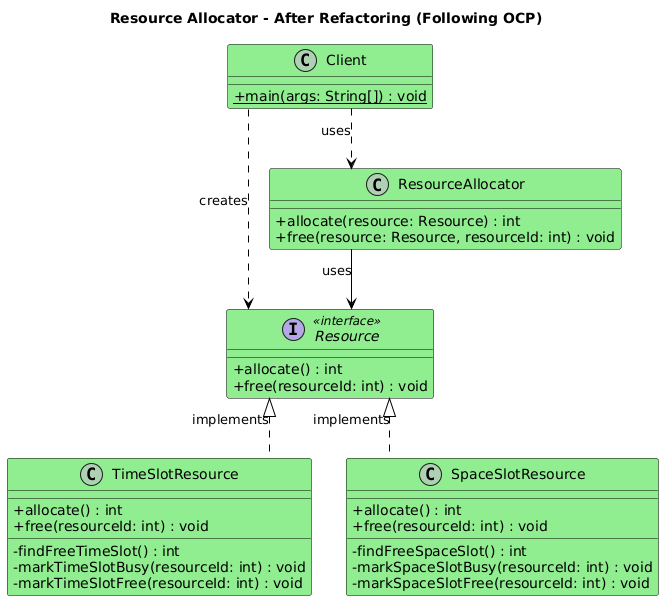
\includegraphics[width=0.9\textwidth]{OCP/plantUML/after.png}
    \caption{UML Diagram - Resource Allocator After Refactoring}
    \label{fig:ocp_after}
\end{figure}

Figure~\ref{fig:ocp_after} illustrates the refactored design where the \texttt{Resource} interface provides abstraction, concrete implementations encapsulate resource-specific logic, and \texttt{ResourceAllocator} depends only on the interface, achieving the Open-Closed Principle.

\subsection{How the Refactoring Aligns with OCP}

The refactored design successfully adheres to the Open-Closed Principle through the following mechanisms:

\subsubsection{Open for Extension}

The system can be extended with new resource types without modifying existing code:

\textbf{Example: Adding a Network Resource}

To add a new network resource type, simply create a new class:

\begin{verbatim}
public class NetworkResource implements Resource {
    @Override
    public int allocate() {
        int resourceId = findFreeNetworkSlot();
        markNetworkSlotBusy(resourceId);
        return resourceId;
    }
    
    @Override
    public void free(int resourceId) {
        markNetworkSlotFree(resourceId);
    }
    
    private int findFreeNetworkSlot() {
        // Network-specific logic
        return 0;
    }
    
    private void markNetworkSlotBusy(int resourceId) {
        System.out.println("Network slot " + resourceId + 
            " marked as busy");
    }
    
    private void markNetworkSlotFree(int resourceId) {
        System.out.println("Network slot " + resourceId + 
            " marked as free");
    }
}
\end{verbatim}

\textbf{No modifications needed to:}
\begin{itemize}
    \item \texttt{Resource} interface
    \item \texttt{ResourceAllocator} class
    \item \texttt{TimeSlotResource} class
    \item \texttt{SpaceSlotResource} class
    \item Any other existing code
\end{itemize}

This demonstrates true extension without modification.

\subsubsection{Closed for Modification}

The core classes remain stable and unchanged:

\begin{table}[H]
\centering
\begin{tabular}{|l|p{9cm}|}
\hline
\textbf{Component} & \textbf{Stability} \\
\hline
Resource Interface & Stable—rarely changes once defined \\
\hline
ResourceAllocator & Stable—no changes needed for new resource types \\
\hline
TimeSlotResource & Stable—changes only if time slot logic changes \\
\hline
SpaceSlotResource & Stable—changes only if space slot logic changes \\
\hline
\end{tabular}
\caption{Component Stability After Refactoring}
\label{tab:ocp_stability}
\end{table}

\subsubsection{Comparison: Before vs. After}

\begin{table}[H]
\centering
\begin{tabular}{|p{5cm}|p{5cm}|p{5cm}|}
\hline
\textbf{Aspect} & \textbf{Before (Violating OCP)} & \textbf{After (Following OCP)} \\
\hline
Adding new resource type & Modify ResourceAllocator, add cases to switch statements, add private methods & Create new class implementing Resource interface \\
\hline
Changes required & 3-4 modifications in existing class & 1 new class, no modifications \\
\hline
Risk of breaking existing code & High—modifying tested code & Low—existing code untouched \\
\hline
Testing requirements & Retest entire ResourceAllocator & Test only new resource class \\
\hline
Code complexity & Increases with each new type & Constant—new types don't add complexity \\
\hline
Coupling & Tight—ResourceAllocator knows all types & Loose—depends on abstraction \\
\hline
Maintainability & Decreases over time & Remains high \\
\hline
\end{tabular}
\caption{Before vs. After Comparison}
\label{tab:ocp_comparison}
\end{table}

\subsubsection{Key Design Patterns Applied}

The refactoring applies several important design patterns:

\begin{itemize}
    \item \textbf{Strategy Pattern:} Different resource allocation strategies encapsulated in separate classes
    \item \textbf{Polymorphism:} Resource-specific behavior achieved through interface implementation
    \item \textbf{Dependency Inversion:} \texttt{ResourceAllocator} depends on \texttt{Resource} abstraction, not concrete types
    \item \textbf{Template Method:} Each resource follows the same allocation pattern but with different implementations
\end{itemize}

\subsubsection{Additional Benefits}

Beyond achieving OCP, the refactored design provides:

\begin{itemize}
    \item \textbf{Improved Testability:}
    \begin{itemize}
        \item Each resource type can be tested independently
        \item Mock resources can be created for testing \texttt{ResourceAllocator}
        \item No need to test all combinations of resource types
    \end{itemize}
    
    \item \textbf{Better Organization:}
    \begin{itemize}
        \item Clear separation of concerns
        \item Each class has a single, well-defined purpose
        \item Easier to navigate and understand the codebase
    \end{itemize}
    
    \item \textbf{Enhanced Reusability:}
    \begin{itemize}
        \item Resource implementations can be reused in different contexts
        \item \texttt{ResourceAllocator} can work with any resource type
        \item Easy to create resource hierarchies or compositions
    \end{itemize}
    
    \item \textbf{Scalability:}
    \begin{itemize}
        \item System can grow indefinitely by adding new resource types
        \item No degradation in code quality as system grows
        \item New developers can add features without understanding entire system
    \end{itemize}
\end{itemize}

\subsection{Real-World Implications}

The Open-Closed Principle has significant implications for real-world software development:

\subsubsection{Version Control and Collaboration}

\begin{itemize}
    \item \textbf{Fewer Merge Conflicts:} Team members can add new features in separate files without conflicting changes
    \item \textbf{Clearer History:} Git history shows new files added rather than complex modifications
    \item \textbf{Easier Code Review:} New extensions are easier to review than modifications to existing code
\end{itemize}

\subsubsection{Continuous Integration/Deployment}

\begin{itemize}
    \item \textbf{Safer Deployments:} New features don't risk breaking existing functionality
    \item \textbf{Faster CI/CD:} Only new code needs extensive testing
    \item \textbf{Incremental Rollout:} New resource types can be deployed gradually
\end{itemize}

\subsubsection{Long-Term Maintenance}

\begin{itemize}
    \item \textbf{Legacy Code Protection:} Well-tested code remains untouched
    \item \textbf{Knowledge Transfer:} New team members can add features without deep system knowledge
    \item \textbf{Technical Debt Reduction:} System doesn't accumulate complexity over time
\end{itemize}

\subsection{Conclusion}

The refactoring from a monolithic \texttt{ResourceAllocator} with \texttt{switch} statements to an interface-based polymorphic design demonstrates the profound impact of the Open-Closed Principle. By ensuring that the system is open for extension but closed for modification, we've created an architecture that:

\begin{itemize}
    \item Scales effortlessly with new requirements
    \item Protects existing, tested code from modification
    \item Reduces the risk of introducing bugs
    \item Improves maintainability and code organization
    \item Facilitates testing and quality assurance
    \item Enables team collaboration without conflicts
    \item Demonstrates professional software engineering practices
\end{itemize}

The transformation illustrates that OCP is not merely a theoretical guideline but a practical approach that leads to more robust, maintainable, and professional software systems. The key insight—\textit{program to interfaces, not implementations}—enables true extensibility while maintaining system stability.
